\label{chap:results}
This chapter discusses the experimental evaluation of SAFE using various control policies, as well as, potential hazards in adaptive mechanisms that can lead to a maladaptive system. We demonstrate here why proactive adaptive systems are needed for massively parallel architectures and why reactive localized adaptive systems will not suffice for future exascale architectures. We additionally demonstrate that fast and accurate collection of pertinent information and quick dispatch of control messages is crucial for convergence toward goals.

First we discuss our experimental setup and then move onto experimental results. Within experimental results, we discuss maladaptation, as well as, working adaptive solutions. For each experiment we discuss the observed behavior and why the behavior occurs. Finally, we provide an overall discussion of the experimental results and the conclusions derived from them.

\section{Experimental Setup}
%{
    This section discusses the experimental setup. Detailed within is the system used to run experiments, the different workloads used, and the different adaptive policies evaluated using said workloads. 
    \subsection{System}
    %{
        For experimental evaluation of adaptive policies within SAFE, we ran on a NUMA quad socket machine with 128 gigabytes of memory and 4 Xeon E5-4610 processors for a total of 24 cores and 48 hardware threads. Because SAFE is an asynchronous multi-threaded simulation framework, the use of parallel processors greatly decreases run time.
    %}
    \subsection{Workloads}
    %{
        \label{sec:workloads}
        In experimentation, we employ synthetic workloads designed to represent various types of operations that might occur during the execution of a program. The first workload type consist of a compute intensive operations individually contributing low amounts of energy, but additively resulting in around a 104 watt load consistently at full operation. While individual instructions themselves differ in terms of energy consumption, the workload is highly stable; and thus useful for demonstrating the maladaptive hazards that can occur in distributed control systems even under highly stable workloads. The second workload type consist of high network energy operations mixed with compute operations. Individually the workload variation may be significant between cores, but collectively on a 2048 core simulation at full operation, variability in power consumption over time is on the order of approximately a 3 watt swing. This workload is useful for demonstrating a maladaptive hazards that can occur under localized adaptive schemes and thus motivating the need for hierarchical adaptive schemes. The third workload is a phased workload consisting of periods of network intensive operations and compute intensive operations. This workload is designed to stress adaptive schemes by introducing a high watt swing between operations over small amounts of time. At full operation, there is about a 90 watt swing at maximum. In essence, this type of workload represents a worse case scenario for adaptive power management schemes in the sense that swings in wattage occur rapidly at very quick intervals. This means that control schemes are more likely to over and under compensate. Other phased workloads would cause similar behavior, but to lesser effect depending on the peaks and dips in wattage. Within an adaptive control system, lower peaks and falls over longer periods of time are much easier to control than quick large oscillations. Our phased workload is used to demonstrate the effectiveness of distributed hierarchical adaptive schemes and why local only adaptive schemes fall short for massively parallel chips. Finally, we demonstrate that hierarchical adaptive schemes can mitigate the presence of maladaptive components within a distributed system; allowing convergence toward a goal not possible with local only adaptive schemes.

        Each workload in the system is run at full frequency and network operation for around 100 microseconds (0.1 seconds) of simulated execution time. This is to stabilize the workload power using a 100 microsecond rolling average of accumulated energy (joules) to compute power (watts). Without this stabilization period, SAFE would not have a valid power window upon which to perform adaptation. After this initial stabilization period, each workload is run for an additional 5000 microseconds (5 seconds) of simulated execution time with adaptive policies enabled. It is during this period of time that we collected wattage and temperature numbers from each simulation that was run. The graphs found in this section reflect the latter time period and exclude the initial stabilization period.
    %}
    \subsection{Policies}
    %{
        \label{sec:policies}
        In terms of policies, localized control engines use a greedy policy that attempts to utilize resources within the goal given. If they are over or under their goal, they will attempt to adjust their block state using the various knobs they have access to. There are two types of adjustments used. The first is to simply throttle individual cores up or down depending on whether they are over or under their goal limit. They will periodically continue to monitor their convergence toward a goal and continue to adjust accordingly. The second is to adjust network activity if it contributes toward their inability to meet a goal. This is implemented in terms of percentages to represent bandwidth tapering. Additionally, if above a certain hard threshold limit and network activity is detected, control engines will immediately throttle network activity to some fraction of full speed in order to mitigate large rises to unsustainable power levels. Eventually, local control engines will converge on a local solution if possible. However, this may not be possible due to the nature of workloads. For example, if their workload is too small to reach a goal limit in the first place, they will be unable to meet the limit. Another example is if control knobs are not fine-grain enough to converge to a local solution. In these situations a local adaptive policy will consistently overshoot and undershoot the goal.

        Higher level control engines on the other hands, do not have direct control over resource usage within the system. These provide goal adjustments to lower lever control engines depending on whether they are above or below their own goal. The net effect is that lower level control engines will begin to converge toward a new goal provided by the higher level engines by using whatever control mechanisms they have. In terms of policies, two simple policies are implemented.
        
        The first policy adjusts the goals of individual lower level control engines in increments of different sizes depending on how far the higher level engine is from its own goal. The exact value of the reduction is configurable. However, the further away from a goal, the larger the adjustment will be. Slight changes will converge more slowly but may converge better; whereas, large values may cause overcompensation and oscillation. The engine upon which a new goal is given is chosen at random. It is worth noting that adjusting the goal of an engine already over its own goal limit may not produce useful results because unless it is maladaptive it is already attempting to meet its power goal, and meeting its own lower level goal may be simply not possible. Ergo, adjusting other engines will likely be more fruitful in practice.
        
        The second policy directs higher level control engines to tally how far they are under their own goal and beneficially adjust goals such that other lower level engines receive portions of the unused goal limit.  This enables components that cannot meet their limit to stop trying and allows those that do meet their limits to run faster if possible. The idea behind this policy is that if control engines are unable to utilize the resources to keep at a particular goal level then it is beneficial to raise other engines goals so that they can increase the utilization of their own resources. Essentially, it allows for more intelligent use of resources within the distributed system.

        All policies use a dampener to mitigate oscillation due to the distributed nature of the control system. This allows adjustment of the rate of control of engines at various levels of the control hierarchy and is configurable by level. Larger dampeners reduce the rate of adjustments and lower dampeners increase the rate of adjustments. In a real system, these rates might be dynamically tuned by an adaptive runtime; however, they are statically configured in these experiments. If no dampener is used, too many changes will occur at once and the resulting feedback information will come too late leading to overshooting of goals, oscillation, and non-convergence; rendering policies ineffective. A dampener that overcompensates will lead to oscillation but with a more predictable pattern.
    %}
%}
\section{Experimental Results}
%{
    This section discusses the experimental results obtained. It is organized by workload type as discussed in Section~\ref{sec:workloads}. For each workload, we demonstrate working adaptive solutions using various policies followed by a discussion of maladaptive behavior that can occur.

    \subsection{Compute Intensive Workload}
    %{
        This section is devoted to a discussion of compute intensive workloads as a case study to demonstrate how adaptive policies may lead to maladaptive behaviors and what the effects are, as well as, the behavior of correct adaptive policies on stable workloads.

        \subsubsection{Adaptive Solutions}
        %{
            \begin{figure}[htb!]
                \centering
                \includegraphics[width=0.82\textwidth]{Fig/compute_graph.pdf}
                \caption[Compute Intensive Workload Using an Adaptive Goal Adjustment Policy with Calibrated Rates (Watts vs Time)]{Shown is the effects of a hierarchical adaptive policy after calibration on a stable compute intensive workload.}
                \label{fig:compute_graph}
            \end{figure}

            If hierarchical decision making processes are working correctly then there should be minimal oscillations and quick convergence toward a goal. For a stable workload, there should be little to no oscillation following the initial convergence period. Figure~\ref{fig:compute_graph} shows the behavior of the calibrated goal adjustment policy on a compute intensive workload. Shown is slight oscillations in activity due to local adaptive engines overcompensating slightly with a collective effect of a slight increase in wattage.
        %}

        \subsubsection{Maladaptive Behaviors}
        %{
            The experiments discussed in this section highlight the various ways in which poor policies within distributed hierarchical adaptive systems can give rise to maladaptive behaviors even for highly regular workloads. Careful calibration of policies needs to be done either by hand or automated in order to avoid such issues. The maladaptive behaviors shown here largely stem from policies either over or under compensating in some way, and resulting in oscillations and non-convergence toward a set goal.

            \begin{figure}[htb!]
                \centering
                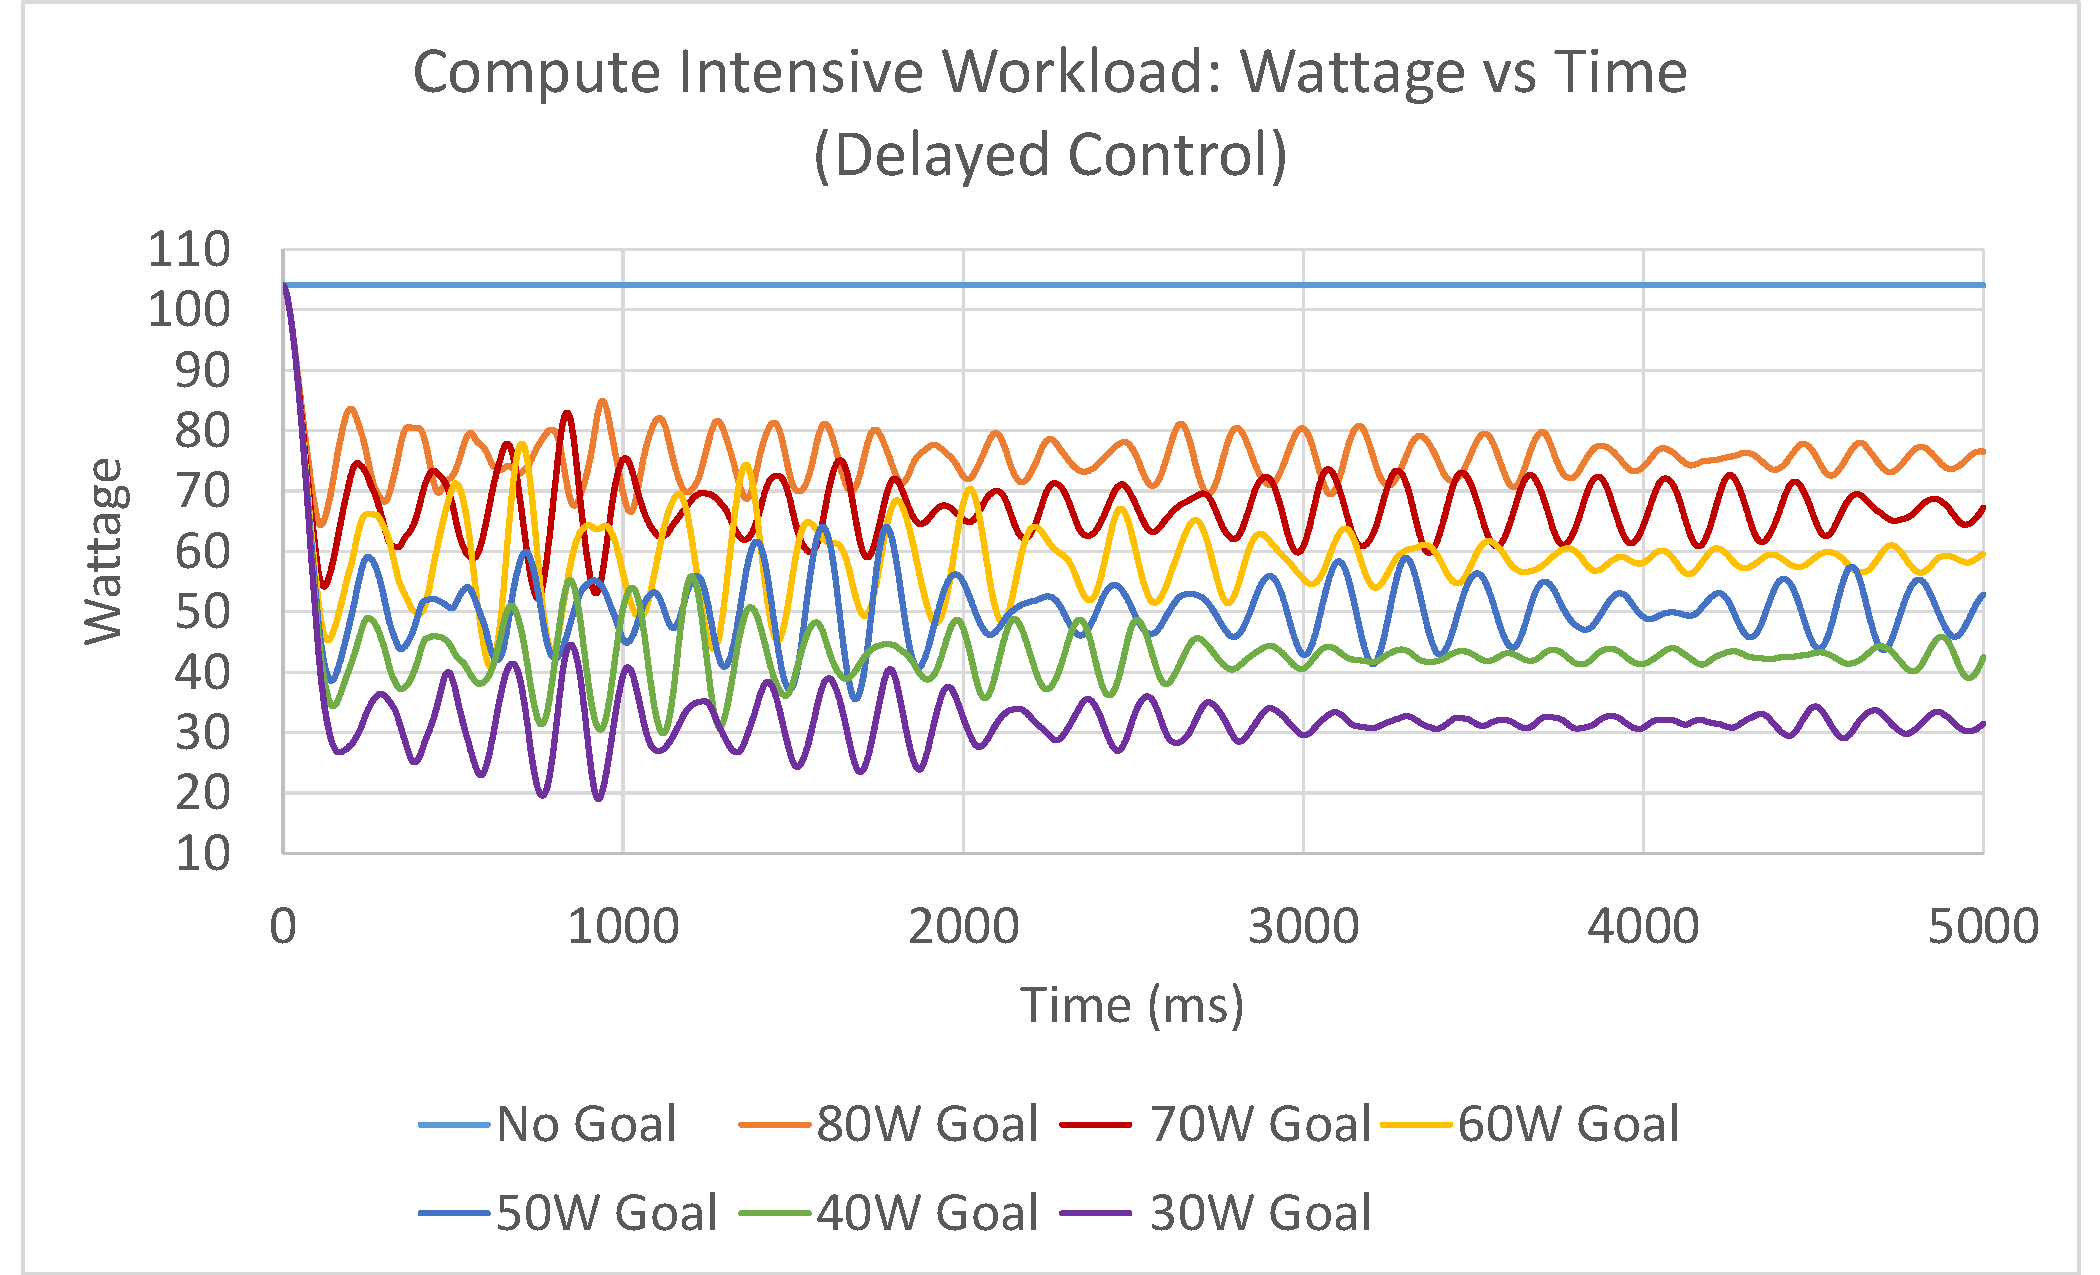
\includegraphics[width=0.82\textwidth]{Fig/compute_delay_graph.pdf}
                \caption[Compute Intensive Workload Using an Adaptive Goal Adjustment Policy with Differing Delayed Control (Watts vs Time)]{Shown is the result of over damping a distributed control policy to adaptively reach a target goal for a stable compute intensive load.}
                \label{fig:compute_delay_graph}
            \end{figure}

            One way in which a distributed hierarchical adaptive system can cause maladaptive behavior is by not quickly enough adapting to state changes. This will result in unpredictable oscillations as shown in figure~\ref{fig:compute_delay_graph}. In a localized adaptive scheme, one might see predictable oscillations if miscalibration of this manner were to occur, but in a distributed system the behavior is more complicated and more difficult to diagnose. The key reason for the unpredictable oscillations is that as the control hierarchy operates independently, control engines will attempt to converge independently of one another leading to differing levels of over compensation at differing points of time.

            In a real system, this behavior could be the result of incorrect information being aggregated up the control hierarchy, information not being passed quickly enough to higher level control engines, the result of control decisions taking too long, or the result of delay in sending control decisions to lower level control engines. It is for this reason that a complicated decision making process involving long computations will not be possible in an massively distributed control engine hierarchy. Decisions must be quick and correct in real time in order to compensate for execution behavior. While offline learning could be used to improve the behavior of adaptive policies, the online components must be calibrated and responsive in terms of (1) receiving up-to-date information, (2) making adaptive decisions, and (3) sending those adaptive decisions down the hierarchy.

            \begin{figure}[htb!]
                \centering
                \includegraphics[width=0.82\textwidth]{Fig/compute_no_delay_graph.pdf}
                \caption[Compute Intensive Workload Using an Adaptive Goal Adjustment Policy with Under Damped Control (Watts vs Time)]{Shown is the result of under damping a distributed control policy to adaptively reach a target goal for a stable compute intensive load.}
                \label{fig:compute_no_delay_graph}
            \end{figure}

            Another way in which a distributed hierarchical adaptive system can cause maladaptive behavior is by making decisions too quickly or not giving enough time for prior decisions to take effect. This will result in predictable patterns as shown in figure~\ref{fig:compute_no_delay_graph}. The characteristic saw tooth pattern seen in the figure is the result of a limit cap on increased power changes over a given time period for the particular policy. In a localized adaptive scheme, an under damped system will result in similarly predictable oscillations depending on the exact policy. In this particular case, only the higher level control engines are over damped, meaning that if the lower level layers of the system were left alone with set goals they would converge to them. However, when the upper level layers of the hierarchy are maladaptive the effects sweep across the system making it unable to effectively adapt.

            In a real system, this behavior could be the result of simply miscalibrated control engines. Another way this might occur is in the event that decisions take a long time to take effect. For example, if a decision is made to power gate a core or block of a real system, it is possible that a delay could occur and that new aggregated data information being sent will not include the effect for some time. A hierarchical decision process needs to be aware of delays in the control knobs that exist in the system in order to effectively adapt. Additionally, predictive proactive policies that account for time delay may be needed to actively adapt if the delay is large. 

            \begin{figure}[htb!]
                \centering
                \includegraphics[width=0.82\textwidth]{Fig/compute_differing_graph.pdf}
                \caption[Compute Intensive Workload Using an Adaptive Goal Adjustment Policy with Differing Rates (Watts vs Time)]{Shown is the result of varying damping rates within a given level in a distributed control policy to adaptively reach a target for a stable compute intensive workload.}
                \label{fig:compute_differing_graph}
            \end{figure}

            A third way in which a distributed adaptive control system can go awry is by differing the control rates of control engines in a maladaptive manner. This behavior is shown in figure~\ref{fig:compute_differing_graph}. This demonstrates that even slightly miscalibrated controllers can cause rippling oscillations throughout the system instead of convergence toward a goal in the presence of a stable workload. While the effect demonstrated is not that bad under stable conditions, it may certainly result in unpredictable behavior in unstable workloads. This highlights the critical need for distributed control systems to be able to identity maladaptive components and mitigate their effects.

            In a real system, this behavior would most likely be the result of simply miscalibrated control engines and only lead to small effects. It is worth noting that such behavior could cause emergent maladaptive behavior that is not detectable within a stable isolated workload. As we will demonstrate with other workloads, maladaptive behavior can cause much worse oscillations within an adaptive system. As such, real systems should provide mechanisms to identity maladaptive components either online or offline in order to provide systems engineers with a clear methodology to fix such issues, as well as, for system software to adapt in the presence of unstable system components.
        %}
    %}
    \subsection{Network Intensive Workload}
    %{
        This section demonstrates effective adaptive policies that generally converge toward a solution for a network intensive goal once given a goal. Additionally, adaptive behavior in the presence of maladaptive components is discussed in detail.

        \subsubsection{Adaptive Solutions}
        %{
            \begin{figure}[htb!]
                \centering
                \includegraphics[width=0.82\textwidth]{Fig/network_goal_adjustment.pdf}
                \caption[Network Intensive Workload Using an Adaptive Goal Adjustment Policy (Watts vs Time)]{Shown is the effect of an adaptive control policy that lowers and raises sub-control engine goals when its goal is not met for a network intensive workload. It is capable of meeting its goal; however, undershoots in some cases possibility due to overcompensating localized control engines.}
                \label{fig:network_goal_adjustment}
            \end{figure}
    
            The experiments discussed in this section show the ability of a hierarchical adaptive system to adapt to a network intensive workload. The two policies used are the adaptive goal adjustment and benefit policies discussed in section~\ref{sec:policies}. These two policies are designed to make minimal adjustments when near a goal and to let lower level control engines converge to a solution with minimal interference when lower level control engines are doing their job effectively. These higher level policies show good behavior both when lower level policies are doing their job and when they aren't. The subsequently discussed experiments show the former case.

            \begin{figure}[htb!]
                \centering
                \includegraphics[width=0.82\textwidth]{Fig/network_benefit.pdf}
                \caption[Network Intensive Workload Using a Benefit Policy (Watts vs Time)]{Shown is the effect of an adaptive control policy that attempts to intelligently reduce slack in load by raising the goal of lower control engines when others fall below their goals. Essentially, it reduces the goal of engines currently below their goal, and increases the goal of other engines.}
                \label{fig:network_benefit}
            \end{figure}

            Figures~\ref{fig:network_goal_adjustment} and~\ref{fig:network_benefit} demonstrate the ability of these policies to converge to a stable solution. The benefit policy is better able to converge to the overall system goal; whereas, the random goal adjustment policy undershoots in some cases. Though, these experiments demonstrate that hierarchical adaptive controls work well during stable network phases, more importantly, the goal adjustment policy is demonstrated to effectively adapt under unstable maladaptive conditions in Section~\ref{sec:network_maladaptive_behaviors} and under phased workloads in Section~\ref{sec:phased}. 
        %}

        \subsubsection{Maladaptive Behaviors}
        %{
            \label{sec:network_maladaptive_behaviors}
            The experiments discussed in this section highlight how limited granularity of control mechanisms can lead to maladaptive behavior, as well as, the effect maladaptive components can have on convergence toward a goal. They also serve to demonstrate how hierarchical control can mitigate some of the effects of maladaptive components.

            \begin{figure}[htb!]
                \centering
                \includegraphics[width=0.82\textwidth]{Fig/network_coarse.pdf}
                \caption[Network Intensive Workload Using an Adaptive Goal Adjustment Policy with Coarse-grain Control (Watts vs Time)]{Shown is the result of providing only coarse grain adaptive network controls to lower level control engines. Network activity is capped to a minimum of 50\% for a network intensive workload.}
                \label{fig:network_coarse}
            \end{figure}

            If controls are too coarse-grained this can lead to the inability to effectively adapt for any control system. Figure~\ref{fig:network_coarse} shows an example of the effects that might occur in such cases. Shown is a network control mechanism that is limited to 50\% of the maximum rate. By capping the limit, the effective minimum wattage of a network intensive workload is around 60 watts because the lowest level control engines can do nothing else to limit activity under the policy. If one were to limit activity to large percentage, 5\% for example, these engines would similarly be unable to meet a goal and would simply oscillate around the goal never converging. While in some sense, this is a unnatural example, it serves to highlight an important point about the granularity of adaptive mechanisms. For example, a real system with hard limits on the granularity of core DVFS states might similarly be unable to meet goals. Instead, cores may oscillate around a goal. As such, the granularity of controls will be a critical aspect in exascale systems.

            \begin{figure}[htb!]
                \centering
                \includegraphics[width=0.82\textwidth]{Fig/network_maladaptive.pdf}
                \caption[Network Intensive Workload Using an Adaptive Goal Adjustment Policy with Maladaptive System Components (Watts vs Time)]{Shown is the result of introducing 64 maladaptive lower level control engines under an adaptive control policy for a network intensive workload. Essentially, the working control engines have mitigated the effects of these other malicious components when possible. In cases such as this, higher level control engines revaluate and assign goals accordingly.}
                \label{fig:network_maladaptive}
            \end{figure}

            Given a distributed system, components may be maladaptive in some way. That is to say, unable to meet a goal for some reason. For example, as discussed above, coarse-grain controls may lead localized control engines to be unable to directly meet a goal. However, in the event of a maladaptive component within the system, a distributed control hierarchy should be resilient enough to detect maladaptive components and minimize the effects; and to meet their own goal if possible. Shown in Figure~\ref{fig:network_maladaptive} is a hierarchical adaptive policy's ability to cope in the event that $\frac{1}{4}$ of components within the system ignore commands and continue operating at maximum frequency and network state. While the system cannot meet a goal below 40 watts, it is perfectly able to converge to a solution for higher goals. This serves as testament to the ability of distributed control engines to cope with maladaption. Local static control policies would simply be unable to cope with such behavior. This is explored in more detail in Section~\ref{sec:phased}.
        %}

    \subsection{Phased Workload}
    %{
        \label{sec:phased}
        This section is devoted to discussion of hierarchical and local adaptation schemes under phased workloads. The particular phased workload, and conditions under which it is run, is designed to stress adaptive schemes, such that, they have a very difficult time converging to an acceptable solution. The central idea is to operate these adaptive schemes under the worst conditions and to demonstrate their effectiveness or non-effectiveness.
        
        \subsubsection{Adaptive Solutions}
        %{
            This section demonstrates effective adaptive solutions for the phased workload. Both wattage and temperature levels for the adaptive goal adjustment policy are shown. As will be denoted below, wattage goals directly translate into temperature goals. The duality of the two is an important aspect not to be understated. 
 
            \begin{figure}[htb!]
                \centering
                \includegraphics[width=0.82\textwidth]{Fig/phase_hier.pdf}
                \caption[Phased Workload Using an Adaptive Goal Adjustment Policy (Watts vs Time)]{Shown is a hierarchical adaptation scheme adapting to a phased workload of local and network operations. Demonstrated is that hierarchical adaptation schemes are capable of effectively mitigating and managing the effects of over and under compensating local control engines.}
                \label{fig:phase_hier}
            \end{figure}

            Figure~\ref{fig:phase_hier} demonstrates that even for highly oscillating workloads consisting of quickly varying phases, hierarchical adaptive schemes are effective and converge to their goal even in the event of a 70 Watt swing at full operation. In this particular case, we see an initial drop in wattage as the scheme takes effect and then a rise and quick convergence. The reason for this behavior is that the policy used immediately drops network activity to a minimum if it is causing control engines to miss their goal by a large amount. As will be demonstrated with subsequent experiments, complete convergence is not possible with static localized schemes and under conditions with maladaptive components, no localized adaptive solution is possible.
            
            \begin{figure}[htb!]
                \centering
                \includegraphics[width=0.82\textwidth]{Fig/phase_hier_temp.pdf}
                \caption[Phased Workload Using an Adaptive Goal Adjustment Policy (Temperature vs Time)]{Shown is a hierarchical adaptation scheme adapting to a phased workload of local and network operations. Demonstrated is that hierarchical adaptation schemes are capable of meeting temperature goals indirectly through wattage goals.}
                \label{fig:phase_hier_temp}
            \end{figure}
            
            Figure~\ref{fig:phase_hier_temp} shows the same phased workload collecting average temperature instead of wattage. It demonstrates that wattage goals necessarily translate into temperature goals. This is due to the nature of average chip temperature levels being the direct result of wattage levels. A hierarchical scheme capable of meeting wattage goals will necessarily be able to meet temperature goals as well. In fact, because temperature changes more slowly than wattage levels, it is easier to for an adaptive scheme to meet temperature goals on average. This is evident when comparing Figure~\ref{fig:phase_hier} to Figure~\ref{fig:phase_hier_temp} where it is shown that temperature levels converge more quickly than wattage and have less variation over time. As such, it is reasonable to expect wattage goals to be used in conjunction with chip specifications to meet a temperature goal instead of directly using temperature goals and temperature machine specific registers. However, this does not preclude using temperature goals directly if so desired. A policy capable of meeting wattage goals within SAFE would need only to collect temperature averages instead of wattage and adapt on those directly. In fact, the aggregation of temperature data is already implemented, but the adaptive policies within SAFE simply use wattage instead. The purpose here is to simply demonstrate that there is a duality between wattage and temperature and that meeting one goal necessarily means meeting the other. Of course, in reality, absolute temperature junction thresholds should always be met. That is to say, if a chip cannot operate above a certain temperature, then built in safe guards should be in place to ensure that it never goes above that temperature outside of higher level system software adaptive schemes. One would expect such a mechanism to be implemented in low level firmware. 
        %}

        \subsubsection{Maladaptive Behaviors}
        %{
            This section demonstrates the effectiveness of hierarchical adaptation under maladaptive conditions, as well as, the behavior of localized adaptation schemes under non-optimal conditions. As will be shown, localized adaptive schemes perform poorly in the presence of maladaptive behavior. 

            \begin{figure}[htb!]
                \centering
                \includegraphics[width=0.82\textwidth]{Fig/phase_local.pdf}
                \caption[Phased Workload Using a Greedy Local Only Adaptive Policy]{Shown is the result of using a localized adaptation scheme with preset goals for adapting a phased workload of local and network operations. Oscillation is present for all goals and convergence toward a stable solution is not guaranteed.}
                \label{fig:phase_local}
            \end{figure}

            Figure~\ref{fig:phase_local} shows the behavior of the phased workload under a statically allocated local adaptive policy. Essentially, what we see is that minor overcompensation by individual control engines leads to oscillations within the system. This reason for this behavior is that though individual overcompensations by themselves are minor, accumulated together, they result in a large wattage swing all at once. Localized adaption schemes cannot mitigate this behavior because they do not have an idea about the current overall wattage state of the system. 

            \begin{figure}[htb!]
                \centering
                \includegraphics[width=0.82\textwidth]{Fig/phase_zoom.pdf}
                \caption[Phased Workload Local Only vs Hierarchal Adaptation (Watts vs Time)]{Shown is a close up view of a local adaptive policy against a hierarchical policy in adapting to a phased workload.}
                \label{fig:phase_zoom}
            \end{figure}

            Figure~\ref{fig:phase_zoom} demonstrates this more clearly by plotting the localized adaptation scheme against the hierarchical scheme discussed above. For a localized adaptive scheme, there are consistently 10 watt swings as the system over and under compensates repeatedly. Where as, the hierarchical adaptive scheme detects and mitigates the trend through the aggregation of data at higher levels of the control hierarchy. Essentially, higher level engines see the large trend that localized schemes are incapable of detecting. This is an important adaptive behavior the spans not only power, but also temperature, or any other system goal. When combined with thousands of individual cores, maladaptive localized behaviors such as these will become a significant problem. The subsequent experiments introducing maladaptive behavior into the control system will demonstrate this even more profoundly.

            \begin{figure}[htb!]
                \centering
                \includegraphics[width=0.82\textwidth]{Fig/phase_local_maladaptive.pdf}
                \caption[Phased Workload Using a Greedy Local Only Adaptive Policy with Maladaptive System Components (Watts vs Time)]{Shown is the result of using a localized adaptation scheme with preset goals for adapting a phased workload of local and network operations in the presence of 64 maladaptive control engines. Extensive oscillation is present for all goals and convergence is not possible due to the nature of localized adaptive schemes to not account for the behavior of other components within a system.}
                \label{fig:phase_local_maladaptive}
            \end{figure}

            \begin{figure}[htb!]
                \centering
                \includegraphics[width=0.82\textwidth]{Fig/phase_hier_maladaptive.pdf}
                \caption[Phased Workload Using an Adaptive Goal Adjustment Policy with Maladaptive System Components (Watts vs Time)]{Shown is a hierarchical adaptation scheme adapting to a phased workload of local and network operations in the presence of 64 maladaptive control engines. Despite an extensive amount of maladaptive components within the system, the control hierarchy does a good job mitigating the effects and demonstrates the resiliency of hierarchical solutions. Convergence toward a solution would be impossible under such conditions with a localized adaptive scheme.}
                \label{fig:phase_hier_maladaptive}
            \end{figure}

            \begin{figure}[htb!]
                \centering
                \includegraphics[width=0.82\textwidth]{Fig/phase_zoom_maladaptive.pdf}
                \caption[Phased Workload Local Only vs Hierarchal Adaptation with Maladaptive System Components (Watts vs Time)]{Shown is a close up view of a local adaptive policy against a hierarchical policy in adapting to a phased workload in the presence of maladaptive system components.}
                \label{fig:phase_zoom_maladaptive}
            \end{figure}

            Figure~\ref{fig:phase_local_maladaptive} shows the same localized adaptation scheme for the phased workload in the presence of $\frac{1}{4}$ of the system exhibiting maladaptive behavior. In this particular case, not only is the system not able to converge to a goal, the localized adaptation scheme results in very large oscillations on the order approximately 40 watts. This behavior is not surprising given that a localized scheme means that well behaved control engines only know about the behavior of components under their control and not other maladaptive sections of the system. But, it highlights an important aspect of adaptive policies within massively scale systems. That is to say, maladaptive components will cause systems to be unable to meet goals without hierarchical adaptive schemes in place.
            
            If we take a look at Figure~\ref{fig:phase_hier_maladaptive}, it shows that even in the presence of large oscillations that result from the maladaptive components, that the hierarchical distributed adaptive schemes perform extremely well considering the conditions under which it is operating. This is shown more clearly in Figure~\ref{fig:phase_zoom_maladaptive} comparing the localized adaptive scheme to the hierarchical adaptive scheme. In one case, the goal is met following small oscillations to convergence and in the other case the goal never met.
    
            In essence, this shows the effectiveness of hierarchical adaptive solutions and makes an argument for the usage of these types of solutions in systems operating at this scale. Demonstrably, localized static schemes will certainly not suffice in cases such as this. With the variability in the operating states of individual cores due to yield, these types of behavior are set to become more common in exascale hardware. Even in cases where the hardware works appropriately, localized maxima and minimas could result in behaviors such as this due to workload patterns or non-optimal localized adaptive engines. Additionally, optimized workloads will certainly result in hot spotting in terms of system resource utilization not shown in these experiments. Static allocation of resources would result in non-optimal solutions not only affecting the wattage as shown here, but also the performance of executing workloads. Ideal adaptive solutions would allocate wattage where needed while converging toward overall system goals.
        %}
    %}
    \subsection{Overall Discussion}
    %{
        Overall, the experimental results demonstrate the need for hierarchical adaptive policies in exascale architectures. Even for relatively stable non-phased workloads, problems meeting goals will occur if individual components are unable to meet their local goal and no higher level adaptive policies are in place to mitigate the effects. In cases with phased workloads, the effects will result in unpredictable behavior due to localized oscillation in different sections of the chip. In conjunction with high levels of maladaptive behavior, this can result in a very large deviation from the specified goal. On other hand, hierarchical adaptive policies are capable of significantly mitigating the effect of maladaptive behavior. Additionally, hierarchical adaptive schemes perform better even when all sections of the system are behaving appropriately in comparison to localized schemes. As discussed earlier in this chapter, this is primarily due to the higher level adaptive engines having a more complete picture of system behavior; and thus, being able correct the overcompensation of localized adaptive engines.

        It is important not to understate the need to maintain a particular granularity of control in terms of adjustable system knobs. As was shown in experimental results, coarse-grain control can lead to an inability for the lower level control engines to meet localized goals. This could simply be the result of an inability to turn off enough components to lower power or temperature to a desired level, or it could be the result of knobs not having enough levels and simply causing oscillations above and below the localized goal. An example of this would be a control engine only capable of switching off an entire block of execution engines at once (8 XEs within SAFE). While higher level adaptive schemes will no doubt mitigate the bad effects of this behavior, the lower level engines may never converge to a solution (depending on their workload); thus causing, jitter and a higher convergence time for higher level system goals.
    %}
%}